\documentclass[a4paper,11pt]{book}
\usepackage[T1]{fontenc}
\usepackage[utf8x]{inputenc}
\usepackage{lmodern}

\usepackage[brazil]{babel}
\usepackage{amsmath,amsfonts,amssymb}
\usepackage{graphicx, xcolor}
\usepackage{array}
\usepackage{relsize}

% tabular
\usepackage{tabularx,color,colortbl}
% tabular

\usepackage{array}
\usepackage{relsize}
% -- hyperlink text
\usepackage[colorlinks,
  urlcolor=blue,
  hyperindex,
  pdfdisplaydoctitle,
  pageanchor,
  linkcolor=blue]{hyperref}
% -- hyperlink text

% -- syntax highlight
\usepackage{minted}
\usemintedstyle{pastie}
% -- syntax highlight
% -- style for bash code
\definecolor{ruleclr}{rgb}{0.95,0.95,0.95}
\newminted[jssnippet]{javascript}{frame=single,tabsize=3}
% -- style for bash code
% -- title pic
\usepackage{titlepic}
% -- title pic

\usepackage[hmargin=3cm,vmargin=3.5cm]{geometry}

\renewcommand\listoflistingscaption{Lista de Códigos-fonte}
\renewcommand\listingscaption{Código-fonte}
\renewcommand{\arraystretch}{1.5} % ajusta altura das linhas das tabelas.
\renewcommand{\labelitemi}{$\blacktriangleright$}
\renewcommand{\labelitemii}{$\triangleright$}
\newcommand{\degree}{\ensuremath{^\circ}}

\definecolor{purple-code}{RGB}{92,53,102}
\definecolor{android-blue}{RGB}{51,181,229}
\definecolor{android-dark-blue}{RGB}{0,153,204}
\definecolor{android-purple}{RGB}{170,102,204}
\definecolor{android-dark-purple}{RGB}{153,51,204}
\definecolor{android-green}{RGB}{153,204,0}
\definecolor{android-dark-green}{RGB}{102,153,0}
\definecolor{android-orange}{RGB}{255,187,51}
\definecolor{android-dark-orange}{RGB}{255,136,0}
\definecolor{android-red}{RGB}{255,68,68}
\definecolor{android-dark-red}{RGB}{204,0,0}

\newcommand{\inlinecode}[1]{
 {\bfseries\ttfamily\textcolor[RGB]{92,53,102}{#1}}}
\newcommand{\menuaction}[1]{
 {\bfseries\ttfamily\textcolor[RGB]{206,92,0}{#1}}}

\usepackage{tikz}
\newcommand*\circled[1]{\tikz[baseline=(char.base)]{
            \node[shape=circle,draw,inner sep=1pt] (char) {#1};}}

% -- glossary
\usepackage[toc=true,style=list]{glossary}

\makeglossary

\storeglosentry{ide}{name=IDE,description={Integrated Development Environment (Ambiente de Desenvolvimento Integrado),
são softwares que auxiliam no desenvolvimento de outros softwares. Ex. NetBeans IDE \url{http://netbeans.org/},
Eclipse IDE \url{http://www.eclipse.org/}}}
\storeglosentry{adt}{name=ADT,description=Android Development Tools (Ferramentas de Desenvolvimento Android)}
\storeglosentry{api}{name=API,description=Application Programming Interface (Interface de Programação de Aplicativos)}
\storeglosentry{jdk}{name=JDK,description={Java Development Kit (Kit de Desenvolvimento Java).
Refere-se ao Java utilizado para desenvolvimento}}
\storeglosentry{sdk}{name=SDK,description=Software Development Kit (Kit de Desenvolvimento de Software)}
\storeglosentry{avd}{name=AVD,description=Android Virtual Device}
\storeglosentry{xml}{name=xml,description={eXtensible Markup Language, foi desenvolvida com o propósito de
estruturar, armazenar e transportar informações.}}
\storeglosentry{ddl}{name=DDL,description={Data Definition Language (Linguagem de Definição de Dados),
é a parte do SQL que permite que as tabelas do banco de dados sejam criadas,
alteradas ou removidas. Ela também define índices (chaves), especifica ligações entre tabelas,
além de impor restrições entre tabelas.}}
\storeglosentry{debug}{name=debug,description={termo utilizado para indicar quais as operações que
estão sendo executadas, verificando assim se estão funcionando como deveria ou se existem defeitos.}}
\storeglosentry{lts}{name=LTS,description={Long Term Support (Termo de Suporte a Longo Prazo), indica
que essa versão terá atualizações por um período de tempo maior, sendo assim você terá um ambiente
estável e sempre atualizado.}}
\storeglosentry{ppa}{name=PPA,description={Personal Package Archives (Pacote de Arquivos Pessoais),
pacotes de terceiros, ou seja, que não são oriundos do repositório oficial do Ubuntu.}}
\storeglosentry{lucid}{name=lucid,description={Codinome utilizado para a versão 10.04 do Ubuntu
(Lucid Lynx)}}
% -- glossary

\title{O Guia Aberto de Android}
\author{Átila Camurça Alves\\2ª Edição}
%\titlepic{
\includegraphics[width=0.6\textwidth]{cover.jpg}}

\begin{document}

% -- title page

\frontmatter

\pagebreak
\thispagestyle{empty}

\begin{figure}[h]
\centering
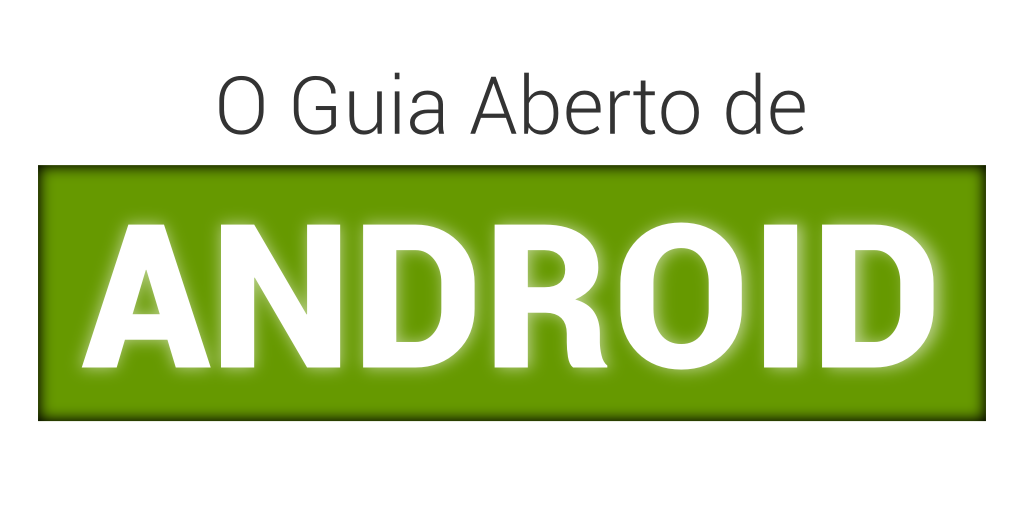
\includegraphics[scale=0.55]{img/guia-aberto-android-front.png}
\end{figure}

\begin{flushright}
% Código para substituir imagem acima caso fique com qualidade baixa
%{\huge O Guia Aberto de}
%
%\vspace{0.2in}
%
%{\Huge \textcolor{android-dark-green}{\textbf{ANDROID}}}
%
%\vspace{0.4in}

{\huge
por Átila Camurça
}

\vspace{1in}

{\Large 2ª Edição}

\vspace{0.2in}

{\small \today}

\vfill
\end{flushright}

\clearpage

\tableofcontents
\listoflistings
\listoftables
\listoffigures

% \chapter*{Prefácio}
% \addcontentsline{toc}{chapter}{Prefácio}
% 
% Lorem ipsum dolor sit amet, consectetur adipiscing elit. Proin vehicula est eu massa auctor consectetur.
% Aenean ante justo, porttitor at porta a, pulvinar eget sapien. Sed feugiat nunc at neque semper mattis ut
% a quam. Nulla lacinia tellus rhoncus nulla placerat iaculis in ac quam. Morbi est lectus, varius eu elementum
% eget, commodo nec velit. Nam suscipit dignissim metus a molestie. Sed tincidunt ullamcorper velit quis faucibus.
% Maecenas adipiscing, elit at pretium vehicula, arcu elit porta justo, vel viverra leo lorem a nisl. Sed
% condimentum placerat ante ac rhoncus. Donec eros massa, hendrerit ac feugiat sit amet, interdum in lorem.
% 
% Nullam mattis auctor enim quis facilisis. Phasellus facilisis ornare neque, et hendrerit mi pharetra in.
% Nunc aliquet mollis est at tempor. Sed porta orci a augue porttitor cursus. Donec sit amet nibh est, quis
% pretium tortor. Quisque mollis metus vulputate lectus blandit consectetur. Mauris tempus mollis tortor, eget
% pulvinar tellus laoreet at. Etiam augue ligula, gravida eget fringilla ut, ultrices sed lacus. Donec turpis est,
% fermentum at tempus id, pharetra ut erat. Cras porttitor, ante nec porta tristique, felis risus luctus nisi, eu
% luctus odio arcu a tortor. Proin elit lacus, sagittis quis lobortis nec, aliquam sed urna. Proin vehicula, sem
% vitae vehicula rhoncus, elit magna tempus mauris, nec mollis sem sem eu est.
% 
% Aliquam egestas aliquet ante non consectetur. Maecenas convallis erat nec arcu varius vel vehicula magna congue.
% Mauris ut tincidunt dui. In interdum lacus eget tortor commodo in aliquet enim adipiscing. Cras eros diam,
% rutrum non facilisis et, adipiscing eu erat. Sed vitae gravida lacus. Integer cursus mollis sem, sed eleifend
% arcu iaculis a. In libero lorem, laoreet ut molestie sed, auctor eu urna. Proin vitae urna sapien, a adipiscing
% dui. Suspendisse eget orci vel est consectetur pharetra. Nullam eu est et augue convallis bibendum faucibus vel
% tortor. Aliquam rutrum tellus sed tortor feugiat et scelerisque eros pulvinar. Sed imperdiet tellus a nunc auctor
% id eleifend nunc luctus. Fusce lacinia, lorem in adipiscing cursus, justo justo sodales enim, nec pretium dolor
% tellus quis quam.
% 
% \pagestyle{plain}

\mainmatter
% capítulos
% -- Preparando o Ambiente de Desenvolvimento
\chapter{Preparando o Ambiente de Desenvolvimento}

\section{Introdução}

O desenvolvimento de aplicativos para a plataforma Android é feito na linguagem Java.
Para esta apostila serão utilizados os seguintes aplicativos e bibliotecas:

% -- TODO: procurar como configurar o mesmo bullet pra todos os itens
\begin{itemize}
	\item Ubuntu 10.04 ou 12.04
	\item Java JDK 6 ou 7
	\item Android SDK
	\item Android 2.2 API 8
	\item Eclipse Juno
	\item ADT Plugin
	\item Sqlite3
	\item Sqliteman
	\item Inkscape
\end{itemize}

Você pode estar se perguntando: ''Por que utilizar essa configuração?''. Bom, para começar
um ambiente de desenvolvimento precisa ser estável, e para isso nada melhor que o
\url{http://releases.ubuntu.com/lucid/} (Ubuntu 10.04) ou ainda o \url{http://releases.ubuntu.com/precise/}
(Ubuntu 12.04) por serem \gls{lts}.

A \gls{ide} Eclipse funciona independente do sistema operacional, então podemos utilizar a versão
mais recente. O mesmo para o plugin \gls{adt}.

Usaremos especificamente para os exemplos a seguir a versão 2.2 do Android. Essa \gls{api} é uma
ótima escolha inicial, pois é a mais utilizada pelos aparelhos mais simples que rodam Android.
É claro que você poderá instalar outras versões e compilar seus aplicativos para \textit{tablets}, etc.

\section{Instalação}

A instalação do Java JDK 6 no Ubuntu 10.04 não é a mesma que no Ubuntu 12.04. Isso porque na época
de lançamento do \gls{lucid}, em 2010, a empresa que desenvolvia o Java era a Sun Microsystems, que
tinha um canal nos repositórios do Ubuntu como parceira (\textit{partner}). Ainda em 2010 a empresa
Oracle comprou a Sun junto com seu software e hardware. Nesse ponto o canal de parceria foi desligado.

Discussões a parte, vamos ver as duas maneiras de instalar o Java.

\subsection{Java JDK 6}

A instalação do Java no Ubuntu 10.04 é bastante simples. Você apenas irá precisar habilitar repositório
de terceiros, ou \textit{Partner}. Isso pode ser feito através do aplicativo \textit{Synaptic}. No menu
principal do Ubuntu clique em \texttt{Sistema $\rightarrow$ Administração $\rightarrow$ Gerenciador de pacotes
Synaptic}.

No menu do Synaptic clique em \texttt{Configuração $\rightarrow$ Repositórios}. Na aba \texttt{Outro Software}
temos vários itens que representam repositórios. Marque os dois repositórios que terminam com \texttt{partner}.
Feche e depois clique em \texttt{Editar $\rightarrow$ Recarregar informações dos pacotes} ou simplesmente
\texttt{Ctrl + R}.

Após a atualização dos pacotes existentes nos repositórios já é possível encontrar o Java \gls{jdk} 6.
No campo de \texttt{Pesquisa rápida} digite: \texttt{sun-java6}. Clique com botão direito no pacote
\texttt{sun-java6-jdk} e selecione a opção \texttt{Marcar para instalação}. Depois basta \texttt{Aplicar}
as mudanças. Para isso clique em \texttt{Editar $\rightarrow$ Aplicar as alterações marcadas} ou \texttt{Ctrl + P}.

\bigskip

Para a instalação no Ubuntu 12.04 temos que habilitar um repositório de terceiros, também conhecido como
\gls{ppa} (Personal Package Archives). Abra um terminal e execute os passos a seguir para adicionar um
repositório e instalar o Java:

\begin{flushleft}\texttt{\$ sudo su\\
\# apt-add-repository ppa:flexiondotorg/java\\
\# apt-get update\\
\# apt-get install sun-java6-jdk\\}
\end{flushleft}

\subsubsection{Um pouco de Linux}

Para quem não está familiarizado com o ambiente Linux vamos a uma pequena explicação. Nos comandos
acima aparecem dois caracteres que não devem ser escritos mas que representam algo importante no âmbito
dos comandos, são eles \texttt{\$} e \texttt{\#}. Estes caracteres indicam qual o nível do usuário;
\texttt{\$} significa usuário comum, \texttt{\#} representa super usuário (\texttt{root}). No comando
\texttt{sudo su} é onde trocamos de usuário comum para super usuário. Neste momento você terá que entrar
com sua senha de \textit{login}.

\subsubsection{Java JDK 7}

Segundo a página de Requerimentos do Sistema (\url{http://developer.android.com/sdk/requirements.html})
do site oficial do Android, é necessário uso do Java 6. Caso você queira utilizar o Java 7, você
terá que configurar seu projeto Android para ser compilado com suporte a versão 6.

A instalação no Ubuntu 12.04 pode ser feita da seguinte maneira:

\begin{flushleft}\texttt{\$ sudo su\\
\# add-apt-repository ppa:webupd8team/java\\
\# apt-get update\\
\# apt-get install oracle-jdk7-installer\\}
\end{flushleft}

Após criar o projeto clique com botão direito do \textit{mouse} em seu projeto e selecione
\texttt{Properties}. Na lista de itens do lado esquerdo selecione \texttt{Java Compiler}. Daí basta clicar
em \texttt{Enable project specific settings} e logo abaixo escolher o nível de compilação em
\texttt{Compiler compliance level}, escolha \texttt{1.6}.

\subsection{Android SDK \label{ssec:sdk}}

Para o Android \gls{sdk} comece pelo \textit{download} \url{http://developer.android.com/sdk/index.html}.

A instalação é feita apenas colocando o SDK em um diretório do sistema. Existem 2 bons locais para
abrigar bibliotecas no Linux, são elas: \texttt{/opt} e \texttt{/usr/local/lib}. Nesse exemplo vamos
utilizar este último. Abra um terminal e vamos aos comandos.

Se você baixou o SDK para seu diretório \textit{Downloads}, proceda da seguinte maneira:

\medskip

\begin{flushleft}
\texttt{\$ cd /home/usuario/Downloads \\
\$ tar -xf android-sdk\b{ }r18-linux.tgz \\
\$ sudo su \\
\# mv android-sdk-linux /usr/local/lib \\
\# cd /usr/local/lib \\
\# ln -s android-sdk-linux android-sdk \\
\# cd android-sdk/tools \\
\# ln -s android /usr/local/bin/android \\
}
\end{flushleft}

\paragraph{Obs.:} troque \texttt{usuario} na primeira linha pelo seu \textit{login} do sistema.

\subsubsection{O poder do Linux}

Dê atenção ao uso do comando \texttt{ln}. Ele é responsável por criar \textit{links} simbólicos. Isso é
muito útil quando se instala um aplicativo ou biblioteca, pois proporciona atualização sem que
outros ajustes sejam feitos. Neste caso basta \textit{linkar} outra vez e pronto.

Note que no último comando temos um link simbólico para o diretório \texttt{/usr/local/bin}. É
nele que colocamos os executáveis globais, ou seja, que são vistos a partir de qualquer outro
diretório. Agora saindo do modo \textit{root} e usando seu próprio usuário instalaremos a API.

\subsection{Android 2.2 API 8}

Ainda no terminal, agora como usuário comum, vamos abrir o aplicativo que instala qualquer uma
das API disponibilizadas pelo Android.

\medskip

\begin{flushleft}
\texttt{\$ android}
\end{flushleft}

\medskip

O aplicativo \texttt{Android SDK and AVD Manager} irá aparecer. Clique em \texttt{Avaliable packages}
e procure pela versão 2.2 API 8 do Android. Selecione e clique em \texttt{Install Selected}. Após
o download você pode verificar a versão instalada em \texttt{Installed packages}, um dos itens é
algo como \texttt{SDK Plataform Android 2.2, API 8, revision 2}.

Se você quiser aproveite para baixar outras versões para utilizar em projetos futuros.

\subsection{Android Virtual Device (AVD)}

Vamos aproveitar e criar nosso \gls{avd} para testar pela primeira vez nosso emulador. Ainda no
\texttt{Android SDK and AVD Manager} clique em \texttt{Virtual devices}, depois em \texttt{New...}

Dê um nome. Você pode usar qualquer nomenclatura, mas é interessante que tenha algo haver com a versão. Assim,
caso você tenha que testar seu código em outras versões você poderá saber qual emulador utilizar. Por
exemplo use \texttt{android-2.2}. Em \texttt{Target} escolha a versão, neste caso
\texttt{Android 2.2 - API Level 8}. Pronto, apenas clique em \texttt{Create AVD}.

\subsubsection{Dicas}

A opção \texttt{Skin} indica qual a resolução da tela do aparelho. Como não é possível
redimensionar a janela, em alguns monitores a janela fica maior que a tela do seu monitor.

A opção \texttt{Snapshot} quando habilitada, serve para salvar o estado do emulador. Isso faz
com que da segunda inicialização em diante se torne mais rápida.

A opção \texttt{SD Card} é ideal caso sua aplicação necessite guardar dados como fotos, arquivos.
O AVD irá reservar um espaço em seu HD permitindo assim o acesso a dados pelo emulador.

\subsection{Eclipse Juno}

O IDE Eclipse pode ser encontrada em \url{http://www.eclipse.org/downloads/}. Para o desenvolvimento
de aplicativos para o Android a versão \texttt{Eclipse IDE for Java Developers} é ideal. Mas se você
tiver interesse em aplicativos Java para Web a opção é baixar a versão \texttt{Eclipse IDE for Java EE Developers}.

Em todo caso as duas vão servir para o desenvolvimento, pois ambas vem com suporte a Java.

O Eclipse não possui instalador, no caso ele já vem pré-compilado. Basta apenas descompactar e executar
o arquivo \texttt{eclipse}.

Para sua comodidade você pode adicionar o Eclipse no menu do Ubuntu. Isso pode ser feito apenas clicando
com o botão direiro do \textit{mouse} no menu principal e escolhendo a opção \texttt{Editar menus}. Ou você pode
usar a dica do blog MAD3 Linux \\ (\url{http://www.mad3linux.org}) - \url{http://va.mu/VSgR}. Essa dica irá
lhe mostrar como adicionar um item ao menu visível a todos os usuários.

\subsection{Plugin ADT}

Para a instalação do plugin ADT vamos abrir o Eclipse, e em seu menu selecione \texttt{Help $\rightarrow$
Eclipse Marketplace...}

Busque por \texttt{adt} e escolha o \texttt{Android Development Tools for Eclipse} da \texttt{Google, Inc.,
Apache 2.0} e clique em \texttt{Install}. O Eclipse irá pedir confirmação sobre os itens a serem instalados,
clique em \texttt{Next}. Agora basta aceitar os termos de uso e clicar em \texttt{Finish}. Após o download
e a instalação, reinicie o Eclipse.

No \texttt{Eclipse Marketplace} você pode encontrar outras ferramentas bastante úteis para um bom desenvolvimento.
Clique na aba \texttt{Popular} e veja as ferramentas mais baixadas, talvez exista uma que você não conheça
mas que sempre precisou.

\subsubsection{Configurando o ADT}

Agora que o plugin foi instalado temos que dizer ao Eclipse onde nós instalamos o Android SDK. Isso
pode ser feito clicando no menu \texttt{Window $\rightarrow$ Preferences}. Selecione \texttt{Android} no painel
lateral esquerdo. Em \texttt{SDK Location} clique em \texttt{Browse...} e indique o diretório do SDK,
caso não lembre, ele está em \texttt{/usr/local/lib/android-sdk}. Clique em \texttt{Apply} na parte inferior
direita para atualizar a lista de API's disponíveis.

Caso você tenha mais dúvidas dê uma olhada na página oficial de instalação do plugin ADT localizada em
\url{http://developer.android.com/sdk/eclipse-adt.html}.

\subsubsection{Testando o ADT \label{sssec:testando}}

Para testar o \texttt{Android Development Tools} ou ADT crie um projeto Android. No menu do Eclipse selecione
\texttt{File $\rightarrow$ New $\rightarrow$ Project...}

Selecione \texttt{Android Application Project} e clique em \texttt{Next}. Dê um nome qualquer ao seu aplicativo,
por exemplo \texttt{hello.android}. Note que o ADT tenta dar um nome ao seu pacote e ao diretório de arquivos
a partir do nome que você digitou. Deixe como está. Em \texttt{Build SDK} é preciso escolher qual API vamos
utilizar, em nosso caso escolha a \texttt{Android 2.2 (API 8)}. Em \texttt{Minimum Required SDK} escolha
a \texttt{API 8: Android 2.2 (Froyo)} indicando que a versão mínima é a \texttt{API 8}. Clique em \texttt{Next}.

Na versão do ADT para o Eclipse Juno, uma novidade apareceu. É possível criar o ícone lançador logo ao criar
o aplicativo. Selecione da maneira que achar melhor e clique em \texttt{Next}. Depois clique em \texttt{Finish}.

Após isso clique com botão direito do \textit{mouse} no projeto recém criado, e \texttt{Run As $\rightarrow$
Android Application}. Se tudo tiver dado certo é possível ver no emulador sua primeira aplicação
rodando.

\subsubsection{Dicas}

Uma vez que você abriu o emulador não o feche. Você irá notar que ao abrir
pela primeira vez ele leva um tempo para isso. Neste caso ao atualizar o código-fonte apenas
rode o aplicativo novamente. O plugin ADT fará com que o aplicativo seja reinstalado no emulador.

Faça o teste com alguns atalhos básicos:
\begin{description}
	\item[Alt + Enter] Maximiza o emulador. Ideal para demostrações.
	\item[Ctrl + F11] Muda a orientação do emulador, retrato ou paisagem.
	\item[F8] Liga/desliga a rede.
\end{description}

Outro elemento essencial é o \texttt{LogCat}. Ele faz parte do ADT e é responsável por mostrar
as mensagens de \textit{log} do emulador. Caso você encontre problemas com seu código o \texttt{LogCat}
será seu melhor aliado. Para acessá-lo no Eclipse clique no menu \texttt{Window $\rightarrow$ Show View
$\rightarrow$ Other...}, clique em \texttt{Android $\rightarrow$ LogCat}.

\subsection{Sqlite3}

Sendo o Sqlite o banco de dados embutido na plataforma Android, nada melhor do que aprendermos um pouco
sobre ele.

O Sqlite é um banco de dados relacional bastante utilizado por dispositivos e sistemas embarcados por
ser leve, robusto, de fácil configuração e, acima de tudo, livre. Para a instalação, abra um terminal
como \texttt{root} e:

\begin{flushleft}
\texttt{\$ sudo su \\
\# apt-get install sqlite3 \\}
\end{flushleft}

Após a instalação é possível utilizar o Sqlite via linha de comando. Faça \textit{logoff} do usuário
\texttt{root} e faça os seguintes testes:

\begin{flushleft}
\texttt{\# exit \\
\$ sqlite \\
SQLite version 2.8.17\\
Enter ".help" for instructions\\
sqlite>\\}
\end{flushleft}

Você deverá ver algo parecido. Para sair utilize o comando \texttt{.exit}. Veja outros detalhes na página
oficial do projeto: \url{http://www.sqlite.org/}.

\subsubsection{Tipos de dados}

Utilize a tabela abaixo para criar suas tabelas futuramente.

\begin{table}[H]
\begin{tabularx}{400pt}{lX}
\hline
\textbf{Nome} & \textbf{Descrição} \\
\hline
\texttt{INTEGER} & valores inteiros, positivos ou negativos. Podem variar de 1 a 8 \textit{bytes}.\\
\texttt{REAL} & valores reais ou decimais.\\
\texttt{TEXT} & usado para armazenar valores, não-limitado. Suporta várias codificações, por exemplo \texttt{UTF-8}.\\
\texttt{BLOB} & objetos binários tais como imagens, arquivos de texto, etc. Também possui tamanho não-limitado.\\
\texttt{NULL} & representa falta de informação.\\
\hline
\end{tabularx}
\caption{Tipos de dados do Sqlite}
\end{table}

\subsection{Sqliteman}

Para uma gerência mais produtiva usaremos o Sqliteman para acessar e modificar bancos de dados. A instalação
é feita via linha de comando. Abra um terminal e:

\begin{flushleft}
\texttt{\$ sudo su\\
\# apt-get install sqliteman\\}
\end{flushleft}

Depois de instalado, acesse o aplicativo do menu principal do Ubuntu em \texttt{Aplicativos $\rightarrow$
Escritório $\rightarrow$ Sqliteman}. Faça alguns testes criando bancos de dados, depois crie algumas tabelas.
Ele possui assistentes que irão auxiliar nos primeiros momentos.

Por exemplo, crie uma base de dados e depois clique com o botão direito do \textit{mouse} em \texttt{Tables}.
Utilize o assistente e veja como é simples criar tabelas no sqlite.

% exemplo_bd.sql
\begin{listing}[H]
  \inputminted[linenos=true,frame=bottomline,tabsize=3]{ sql }{ source/exemplo-bd-1.sql }
  \caption{Exemplo de banco de dados [exemplo-bd.sql]}
\end{listing}

Observe que podemos fazer auto-relacionamento na tabela. Assim somos capazes de executar a seguinte SQL,
contando o número de distros que derivam de uma outra original. Veja:

% exemplo_bd.sql
\begin{listing}[H]
  \inputminted[linenos=true,frame=bottomline,tabsize=3]{ sql }{ source/exemplo-bd-2.sql }
  \caption{Exemplo de \textit{query} com \textit{subquery} [exemplo-bd.sql]}
\end{listing}

Mais informações em: \url{http://sqliteman.com/}

\subsection{Inkscape}

Uma ótima ferramenta de desenho vetorial é o Inkscape. Ela será bastante útil pois o desenvolvimento
de aplicativos hoje em dia é baseado muito em figuras para facilitar a navegação, identidade visual,
entre outras coisas.

A instalação é feita de forma simples. Num terminal:

\begin{flushleft}
\texttt{\$ sudo su\\
\# apt-get install inkscape\\}
\end{flushleft}

Para dicas de como criar ícones para os diversos elementos do Android veja a página
\url{http://developer.android.com/design/style/iconography.html}.


% -- Exemplo Prático
\chapter{Exemplo prático}

\section{Primeira aplicação - Contatos}

Crie uma nova aplicação chamada \textbf{Contatos}. Para o nome do pacote use \inlinecode{contatos.app}.
Chame a \texttt{Activity} de \texttt{MainActivity}, que será responsável pela Atividade Principal. Depois
configure a plataforma Android a ser utilizada e \texttt{Finish} (em caso de dúvida verifique o item
\ref{sssec:testando} Testando o ADT).

Essa pode não ser uma aplicação muito útil, mas com ela poderemos aprender como funciona o Android. Você
só poderá criar algo se você souber utilizar as ferramentas.

\subsection{AndroidManifest.xml}

Esse é o arquivo que define nossa aplicação, mapeia as \texttt{Activity}'s, entre outras configurações. Ao finalizar
a criação do projeto, inicialmente este arquivo deverá conter o seguinte conteúdo:

% AndroidManifest.xml
\begin{listing}[H]
  \inputminted[linenos=true,frame=bottomline,tabsize=3]{ xml }{ source/AndroidManifest-1.xml }
  \caption{Projeto inicial [AndroidManifest.xml]}
\end{listing}

\subsection{Activity\label{ssec:act}}

Não existe método \inlinecode{main} visível ao programador no Android. Ao invés disso temos \texttt{Activity}'s.
Para que o Android saiba qual ele deve iniciar primeiro utilizamos um \texttt{intent-filter} como visto
no trecho de código acima da linha \circled{09} a \circled{12}.
Para nossa primeira \texttt{Activity} criaremos uma lista de contatos e um menu para criação de novo contato.

Para construir o layout inicial de nossa aplicação precisamos editar o arquivo \texttt{main.xml} localizado em
\texttt{res/layout}.

% res/layout/main.xml
\begin{listing}[H]
  \inputminted[linenos=true,frame=bottomline,tabsize=3]{ xml }{ source/main-1.xml }
  \caption{Layout principal [res/layout/main.xml]}
\end{listing}

Deste momento em diante tenha em mente que os arquivos \texttt{\gls{xml}} aqui descritos são apenas para
você poder comparar e ver se não esqueceu nada. Todos os \textit{layout}'s devem ser criados usando a
ferramenta ADT. Você irá notar que ao abrir o \texttt{xml} uma janela de \textit{layout} aparecerá.
Para visualizar o \texttt{xml} ou o \textit{layout} gráfico basta utilizar a aba inferior esquerda.

Por fim, temos o menu. Clique com o botão direito do \textit{mouse} em seu projeto e \texttt{New
$\rightarrow$ Other...} ou \texttt{Ctrl + N}. Procure por \texttt{Android XML File}. Em \texttt{Resource
Type} escolha a opção \texttt{Menu}. Chame-o de \texttt{main\b{ }menu.xml}.

% res/menu/main_menu.xml
\begin{listing}[H]
  \inputminted[linenos=true,frame=bottomline,tabsize=3]{ xml }{ source/main_menu-1.xml }
  \caption{Menu principal [res/menu/main\b{ }menu.xml]}
\end{listing}

Pronto, já temos nosso layout. Compile o projeto e vamos a próxima iteração.

\subsubsection{Convenção de nomes para ícones\label{sssec:nomeicones}}

Observe que o ícone utilizado no menu vem junto com o SDK do Android. Você pode visualizar os
ícones em \texttt{SDK\b{ }INSTALL/plataforms/android-8/data/res/drawable-hdpi}
(substitua \texttt{SDK\b{ }INSTALL} pelo diretório de instalação do SDK do Android, no nosso caso
\texttt{usr/local/lib/android-sdk}, \ref{ssec:sdk}). Note que há \textit{namespaces} ou prefixos em
cada um dos ícones. O Android recomenda a seguinte convenção:

\begin{table}[H]
\begin{tabularx}{440pt}{lXX}
\hline
\textbf{Tipo de Recurso} & \textbf{Prefixo} & \textbf{Exemplo} \\
\hline
Ícones & \texttt{ic\b{ }} & \texttt{ic\b{ }adicionar.png}\\
Launcher icons & \texttt{ic\b{ }launcher\b{ }} & \texttt{ic\b{ }launcher\b{ }calendario.png}\\
Menu e Action Bar & \texttt{ic\b{ }menu\b{ }} & \texttt{ic\b{ }menu\b{ }ajuda.png}\\
Status bar icons & \texttt{ic\b{ }stat\b{ }notify\b{ }} & \texttt{ic\b{ }stat\b{ }notify\b{ }msg.png}\\
Tab icons & \texttt{ic\b{ }tab\b{ }} & \texttt{ic\b{ }tab\b{ }recente.png}\\
Dialog icons & \texttt{ic\b{ }dialog\b{ }} & \texttt{ic\b{ }dialog\b{ }info.png}\\
\hline
\end{tabularx}
\caption{Convenção para nome dos ícones}
\end{table}

Note que você não é obrigado a utilizar os prefixos citados acima, isto é apenas uma convenção.
Veja mais detalhes em \url{http://developer.android.com/guide/practices/ui_guidelines/icon_design.html}.

Abra o arquivo \texttt{MainActivity.java} e vá ao método \inlinecode{onCreate}. Defina o \textit{layout} como
sendo nosso \texttt{main.xml}. Para isso adicione o \textit{layout} \textbf{main} ao final do método:

% MainActivity.java
\begin{listing}[H]
  \inputminted[linenos=true,frame=bottomline,tabsize=3]{ java }{ source/MainActivity-1.java }
  \caption{Definir layout [MainActivity.java]}
\end{listing}

\paragraph{Cuidado:\label{par:r}} no ambiente Android temos uma classe chamada \texttt{R}. Ela existe tanto
na biblioteca do Android como em cada projeto. Nesse caso faça o \textit{import} da classe
\texttt{contatos.app.R}. A classe \texttt{android.R} é utilizada em outras situações, onde códigos
pré-prontos foram disponibilizados pela equipe do Android.

Agora precisamos sobrescrever os métodos \inlinecode{onCreateOptionsMenu} e \inlinecode{onOptionsItemSelected}.
Eles irão criar o menu a partir de nosso \textit{layout} e notificar quando os itens do menu forem
pressionados, respectivamente. Vamos ao código:

% MainActivity.java
\begin{listing}[H]
  \inputminted[linenos=true,frame=bottomline,tabsize=3]{ java }{ source/MainActivity-2.java }
  \caption{Criando o menu [MainActivity.java]}
\end{listing}

\subsection{Formulários}

Agora vamos criar nosso formulário para criação e edição de contatos. Começaremos pelo \textit{layout}.
Crie um arquivo \texttt{xml} em \texttt{res/layout} chamado \texttt{salvar.xml}.

Existem alguns pontos importantes para este trecho de código. Começando pelo \textit{layout} inicial,
onde usaremos \texttt{TableLayout}. Esse \textit{layout} é ideal para telas com estilo tabela.

Um detalhe importante para observarmos neste \textit{layout} é que ele possui o atributo
\texttt{stretchColumns} com valor \texttt{1}. Isso quer dizer que a coluna \texttt{1} da tabela
terá o maior tamanho possível, respeitando o tamanho mínimo das outras células. Para visualizar as mudanças
você pode tentar usar outros valores como \texttt{0} tornando a primeira coluna maior que as demais,
ou ainda \texttt{*} que fará com que todas as células tenham o mesmo tamanho.

% res/layout/salvar.xml
\begin{listing}[H]
  \inputminted[linenos=true,frame=bottomline,tabsize=3]{ xml }{ source/salvar-1.xml }
  \caption{Formulário principal [res/layout/salvar.xml]}
\end{listing}

Crie uma nova \texttt{Activity} chamada \texttt{SalvarActivity} dentro de \texttt{contatos.app.view}.
Para irmos de uma \texttt{Activity} para outra precisamos de um \texttt{Intent}. Um de seus construtores recebe
como parâmetros a instância da classe em que estamos, sendo que ela deve implementar a interface \texttt{Context}
e o nome da classe a qual deve ser mostrada. Veja como implementar o método \inlinecode{irParaSalvar}
da classe \texttt{MainActivity}:

% MainActivity.java
\begin{listing}[H]
  \inputminted[linenos=true,frame=bottomline,tabsize=3]{ java }{ source/MainActivity-3.java }
  \caption{Mudando de Activity [MainActivity.java]}
\end{listing}

Veremos agora como manipular \texttt{EditText}'s, que representam os campos de entrada de dados. Abra o
\texttt{SalvarActivity} e adicione o método \inlinecode{carregar} e crie atributos para guardar os \texttt{EditText}'s:

% SaveActivity.java
\begin{listing}[H]
  \inputminted[linenos=true,frame=bottomline,tabsize=3]{ java }{ source/SalvarActivity-1.java }
  \caption{Utilizando EditText's [SalvarActivity.java]}
\end{listing}

Para que a \texttt{Activity} funcione precisamos mapeá-la no arquivo \texttt{AndroidManifest.xml}. Adicione o
conteúdo abaixo entre as \textit{tags} \texttt{application}:

% AndroidManifest.xml
\begin{listing}[H]
  \inputminted[linenos=true,frame=bottomline,tabsize=3]{ xml }{ source/AndroidManifest-2.xml }
  \caption{Mapear SalvarActivity [AndroidManifest.xml]}
\end{listing}

Utilize sempre o ADT e apenas confira se o arquivo está da maneira correta.

\subsection{Construindo o Model da aplicação\label{ssec:model}}

Precisamos de um \textit{helper} para fazer acesso ao banco de dados. O Android provê suporte
a bancos de dados Sqlite por padrão. Qualquer banco de dados que você criar será acessível pelo nome
por qualquer classe na sua aplicação, mas não fora dela.

Crie uma classe chamada \texttt{ContatoHelper} em \texttt{contatos.app.model} que extende de
\texttt{SQLiteOpenHelper}. Essa classe será capaz de ler e escrever no banco de dados graças aos métodos 
\inlinecode{getReadableDatabase()} e \inlinecode{getWritableDatabase()}, respectivamente.

A princípio temos que criar um construtor passando como parâmetros o nome do banco de dados e a versão
da \gls{ddl}. Logo em seguida precisamos implementar os métodos \inlinecode{onCreate}, no qual iremos
criar as tabelas e \inlinecode{onUpdate}, caso tenhamos que alterar alguma tabela.

% ContatoHelper.java
\begin{listing}[H]
  \inputminted[linenos=true,frame=bottomline,tabsize=3]{ java }{ source/ContatoHelper-1.java }
  \caption{Helper da aplicação [ContatoHelper.java]}
\end{listing}

Para a iteração de criação de um novo contato, ainda em \texttt{ContatoHelper} vamos adicionar um método
\inlinecode{criar}. Faça:

% ContatoHelper.java
\begin{listing}[H]
  \inputminted[linenos=true,frame=bottomline,tabsize=3]{ java }{ source/ContatoHelper-2.java }
  \caption{Criar novo contato [ContatoHelper.java]}
\end{listing}

Agora temos que fazer a chamada do método \inlinecode{criar} da classe \texttt{ContatoHelper} em
\texttt{SalvarActivity}. Para isso temos que criar uma instância de \texttt{ContatoHelper}, adicionar
o botão salvar e adicionar um \textit{Listener} de \textit{click} (faça o \textit{import}
da classe\\ \texttt{android.view.View.OnClickListener}). Vamos ao código:

% SaveActivity.java
\begin{listing}[H]
  \inputminted[linenos=true,frame=bottomline,tabsize=3]{ java }{ source/SalvarActivity-2.java }
  \caption{Fim da iteração criar contato [SalvarActivity.java]}
\end{listing}

Com essa implementação já é possível salvar contatos na base de dados.

\subsection{Mostrando os dados na View\label{ssec:listview}}

Após salvar os dados no banco, devemos ser capazes de obter tais informações e colocá-las em forma
de Lista. Para isso criaremos um novo \textit{layout} que será responsável por representar uma linha
de nossa Lista. Essa linha deve ser semelhante a figura abaixo:

\begin{figure}[h]
\centering
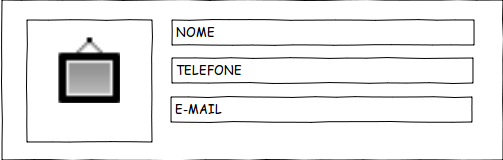
\includegraphics[scale=0.6]{img/layout-linha.png}
\caption{Layout linha da Lista}
\end{figure}

Para isso crie um arquivo chamado \texttt{linha.xml} em \texttt{res/layout} com o seguinte conteúdo.
% -- TODO: exemplificar o trecho de código.

% res/layout/linha.xml
\begin{listing}[H]
  \inputminted[linenos=true,frame=bottomline,tabsize=3]{ xml }{ source/linha-1.xml }
  \caption{Layout para cada linha da lista [res/layout/linha.xml]}
\end{listing}

Agora vamos até \texttt{ContatoHelper} e adicionar o método \inlinecode{listar}. E também adicionaremos
métodos para facilitar obter os valores de cada atributo.

% ContatoHelper.java
\begin{listing}[H]
  \inputminted[linenos=true,frame=bottomline,tabsize=3]{ java }{ source/ContatoHelper-3.java }
  \caption{Listar contatos existentes [ContatoHelper.java]}
\end{listing}

Para popular cada linha de nossa Lista vamos criar uma classe interna (\textit{inner class}) em
\texttt{MainActivity}. Assim podemos fazer \textit{cache} dos objetos aumentando a performance.
Use o sufixo \texttt{Holder} para esse tipo de classe.

% MainActivity.java
\begin{listing}[H]
  \inputminted[linenos=true,frame=bottomline,tabsize=3]{ java }{ source/MainActivity-4.java }
  \caption{Classe Holder [MainActivity.java]}
\end{listing}

Levando em conta que estamos usando a interface \texttt{Cursor} em nosso \texttt{Helper} temos
que criar uma classe que extende de \texttt{CursorAdapter} que será responsável por definir o
\textit{layout} de cada linha da Lista. Crie uma classe interna chamada \texttt{ContatoAdapter}.
Iremos sobrescrever dois métodos, \inlinecode{newView()} e \inlinecode{bindView()}, que são responsáveis
por inflar (\textit{inflate}) uma nova linha e reciclar uma linha existente, respectivamente.

% MainActivity.java
\begin{listing}[H]
  \inputminted[linenos=true,frame=bottomline,tabsize=3]{ java }{ source/MainActivity-5.java }
  \caption{Classe Adapter [MainActivity.java]}
\end{listing}

Com a introdução do \texttt{Helper} teremos que criar uma instância da classe \texttt{Cursor}
para popular nossa \texttt{ListView}. Vamos ao código-fonte:

% MainActivity.java
\begin{listing}[H]
  \inputminted[linenos=true,frame=bottomline,tabsize=3]{ java }{ source/MainActivity-6.java }
  \caption{Popular ListView [MainActivity.java]}
\end{listing}

Nunca esquecendo de fechar o \texttt{helper} ao sair, pois assim garantimos que a conexão com
o banco será fechada.

\subsection{Editando dados existentes\label{ssec:edit}}

Para a edição de informações usaremos o mesmo \texttt{Activity} do criar, ou seja, \texttt{SalvarActivity}.
Para isso precisamos passar um parâmetro para o \texttt{Activity}. Usaremos então um método do
\texttt{Intent} que é responsável por isso, \inlinecode{putExtra(chave, valor)}.

Para uma passagem de parâmetros segura devemos usar um \textit{namespace} para que não colida com
nenhum nome já utilizado pelo Android. Para isso criaremos uma variável estática do tipo \texttt{String}.
Isso acontecerá quando o usuário pressionar a linha que ele deseja editar. Podemos fazer isso utilizando
a interface \texttt{OnItemClickListener}.

Vamos incrementar também o método \inlinecode{irParaSalvar} passando o parâmetro caso haja um. Vamos ao
código:

% MainActivity.java
\begin{listing}[H]
  \inputminted[linenos=true,frame=bottomline,tabsize=3]{ java }{ source/MainActivity-7.java }
  \caption{Passagem de parâmetros [MainActivity.java]}
\end{listing}

Agora é hora de tratar nosso parâmetro no \texttt{SalvarActivity}. Caso haja um parâmetro precisamos
obter os dados existentes no banco de dados para então editá-lo. Neste caso precisaremos de mais dois
métodos em \texttt{ContatoHelper}, que são \inlinecode{ler} e \inlinecode{atualizar}.

% ContatoHelper.java
\begin{listing}[H]
  \inputminted[linenos=true,frame=bottomline,tabsize=3]{ java }{ source/ContatoHelper-4.java }
  \caption{Ler e atualizar dados existentes [ContatoHelper.java]}
\end{listing}

O próximo passo é tratar no \texttt{SalvarActivity} caso o parâmetro tenha sido enviado ou não. Caso positivo
devemos carregar os dados existentes no banco de dados e depois atualizá-los.

% SaveActivity.java
\begin{listing}[H]
  \inputminted[linenos=true,frame=bottomline,tabsize=3]{ java }{ source/SalvarActivity-3.java }
  \caption{Usando Activity para criar ou atualizar [SalvarActivity.java]}
\end{listing}


\chapter{Livro de Receitas}

\section{Mostrando Diálogos}

No Android podemos criar diálogos no \texttt{Activity} mostrando opções ao usuário, como por exemplo,
escolher itens de uma lista, ou responder sim ou não a uma ação, etc.

Vamos incrementar algumas partes de nosso código e tentar encaixar algumas funcionalidades
relacionadas.

\subsection{Editar/Excluir ao clicar e segurar na ListView}

Vamos implementar uma ação comum no mundo Android, que ao clicar e segurar num item
da \texttt{ListView}, ele mostra opções editar e excluir, por exemplo. Isto pode ser
feito facilmente usando \texttt{AlertDialog.Builder}, uma classe com métodos pré-prontos
para serem usados por você.

Neste exemplo precisaremos editar \texttt{ContatoHelper} e adicionar um método para
deletar um contato, editar nosso \texttt{MainActivity} no método \inlinecode{configurar}
e adicionar um \textit{Listener} que ao clicar e segurar num item da \texttt{ListView}
um método é acionado. Vamos a implementação:

% ContatoHelper.java
\begin{listing}[H]
  \inputminted[linenos=true,frame=bottomline,tabsize=3]{ java }{ source/ContatoHelper-5.java }
  \caption{Deletar dados existentes [ContatoHelper.java]}
\end{listing}

% MainActivity.java
\begin{listing}[H]
  \inputminted[linenos=true,frame=bottomline,tabsize=3]{ java }{ source/MainActivity-8.java }
  \caption{Adicionar Listener para click longo [MainActivity.java]}
\end{listing}

Note a necessidade de um novo método em \texttt{MainActivity}, o \inlinecode{exibirMensagem}.
Ele é bastante útil quando se quer exibir uma mensagem rapidamente e depois ela suma.
Para isso usamos a classe \texttt{Toast}.

\subsection{Diálogo de confirmação}

Deletar algo é uma coisa que deve ser feita com cuidado, então sempre é bom confirmar com
o usuário se ele deseja realmente deletar um contato. Para isso usaremos o \texttt{AlertDialog.Builder}
mais uma vez, agora apenas com uma mensagem e os botões \textit{Sim} ou \textit{Não}.


Ainda em \texttt{MainActivity} criaremos um outro \texttt{AlertDialog.Builder} no momento que o usuário
clicar em \texttt{Deletar}. Segue o trecho:

% MainActivity.java
\begin{listing}[H]
  \inputminted[linenos=true,frame=bottomline,tabsize=3]{ java }{ source/MainActivity-9.java }
  \caption{Diálogo de confirmação ao deletar contato [MainActivity.java]}
\end{listing}

Pronto, agora o trecho que deleta o contato foi movido para dentro do \textit{Listener} do botão
\textit{Sim}. No botão \textit{Não} passamos \texttt{null} no \textit{Listener}, pois caso
seja a opção escolhida apenas fazemos nada. Você pode se quiser criar um \textit{Listener} e mostrar
uma mensagem do tipo, \textit{Cancelado pelo usuário}, para isso usando o método \inlinecode{exibirMensagem}.

% DONE: fazer validação do telefone e do e-mail

\subsection{Entrada de diferentes tipos de dados}

O Android foi desenvolvido com muitos recursos pré-prontos para facilitar o desenvolvimento de aplicações.
Um recurso bastante útil é a distinção dos dados que irão ser inseridos nos \texttt{TextView}'s. Com isso
o teclado virtual do cliente se adapta ao tipo de dado que será inserido. No nosso caso faremos distinção
do campo \texttt{telefone}, onde apenas números e hífens(-) podem ser inseridos, e o campo \texttt{e-mail}
onde a presença do arroba(@) e pontos(.) são elementos essenciais.

Vejamos alguns valores aceitos pelo \texttt{inputType}:

\begin{itemize}

  \item Para textos:
  \begin{itemize}
    \item text
    \item textCapCharacters
    \item textMultiLine
    \item textUri
    \item textEmailAddress
    \item textPersonName
    \item textPassword
    \item textVisiblePassword
  \end{itemize}

  \item Para números:
  \begin{itemize}
    \item number
    \item numberSigned
    \item numberDecimal
    \item phone
    \item datetime
    \item date
    \item time
  \end{itemize}

\end{itemize}

Precisaremos alterar apenas o \texttt{salvar.xml} localizado em \texttt{res/layout}. Localize o atributo
\texttt{inputType} dos campos \texttt{telefone} e \texttt{e-mail} e altere os valores da seguinte maneira:

% res/layout/salvar.xml
\begin{listing}[H]
  \inputminted[linenos=true,frame=bottomline,tabsize=3]{ xml }{ source/salvar-2.xml }
  \caption{Distinção de dados [res/layout/salvar.xml]}
\end{listing}

\subsection{Validação de dados}

Mesmo configurando um \texttt{inputType} para seu \texttt{TextView} pode não ser o bastante para que
os dados inseridos estejam corretos. Para isso usaremos a classe \texttt{Patterns} do pacote
\texttt{android.util}. Nela podemos encontrar alguns objetos bastante úteis na hora de validar
dados. Entre eles estão os objetos \texttt{Patterns.EMAIL\b{ }ADDRESS} e \texttt{Patterns.PHONE}. Com
eles podemos validar de forma simples os dados inseridos em nosso formulário.

Em nosso \texttt{SalvarActivity} adicionaremos um método \inlinecode{validar} passando como parâmetro
um \texttt{Contato}. Copie o método \inlinecode{exibirMensagem} da classe \texttt{MainActivity} para
mostrar uma mensagem caso alguma validação seja falsa.

\paragraph{OBS:} Para um melhor reuso crie uma classe abstrata que implementa o método \inlinecode{exibirMensagem}
e que extenda de \texttt{Activity} e faça com que seus \texttt{Activity}'s herdem dela. É uma boa
prática.

Vamos ao trecho de código:

% SaveActivity.java
\begin{listing}[H]
  \inputminted[linenos=true,frame=bottomline,tabsize=3]{ java }{ source/SalvarActivity-4.java }
  \caption{Validação dos dados [SalvarActivity.java]}
\end{listing}

% DONE: fazer com que ao clicar e segurar fazer uma chamada ou enviar e-mail para o contato.
\subsection{Fazendo uma ligação}

Já que estamos fazendo uma lista de contatos nada melhor que usar o número do telefone dos
contatos inseridos para realizar chamadas. Para isso vamos aprender um pouco sobre \textbf{Permissões}.

Permissões no Android são definidas no \texttt{AndroidManifest.xml}. Ao instalar seu aplicativo,
o usuário saberá quais as permissões que o seu aplicativo necessita para ser executado.

Por padrão, o Android traz uma série de permissões que auxiliam seu aplicativo a se comunicar com
o aparelho. Abaixo alguns exemplos:

\begin{itemize}
\item Verificação
\begin{itemize}
  \item \texttt{ACCESS\b{ }NETWORK\b{ }STATE}
  \item \texttt{ACCESS\b{ }WIFI\b{ }STATE}
  \item \texttt{BATTERY\b{ }STATS}
\end{itemize}

\item Comunicação
\begin{itemize}
  \item \texttt{BLUETOOTH}
  \item \texttt{CALL\b{ }PHONE}
  \item \texttt{INTERNET}
  \item \texttt{SEND\b{ }SMS}
\end{itemize}

\end{itemize}

A lista completa pode ser vista em 
\url{http://developer.android.com/reference/android/Manifest.permission.html}.\\

Edite o \texttt{AndroidManifest.xml} e adicione a permissao \texttt{CALL\b{ }PHONE}.

% AndroidManifest.xml
\begin{listing}[H]
  \inputminted[linenos=true,frame=bottomline,tabsize=3]{ xml }{ source/AndroidManifest-3.xml }
  \caption{Permissão de realizar chamadas [AndroidManifest.xml]}
\end{listing}

Agora vamos adicionar um item ao diálogo que aparece ao clicar e segurar um item da \texttt{ListView}.
Ele servirá para implementarmos o trecho que realiza a chamada. Vamos a ele:

% MainActivity.java
\begin{listing}[H]
  \inputminted[linenos=true,frame=bottomline,tabsize=3]{ java }{ source/MainActivity-10.java }
  \caption{Item chamar no diálogo [MainActivity.java]}
\end{listing}

\newpage

\subsection{Enviando e-mail}

Para envio de e-mail você pode simplesmente usar a aplicação de e-mail padrão do aparelho.
Seguindo o mesmo princípio do exemplo anterior vamos apenas inserir um trecho de código
no método \inlinecode{configurar} da classe \texttt{MainActivity}:

% MainActivity.java
\begin{listing}[H]
  \inputminted[linenos=true,frame=bottomline,tabsize=3]{ java }{ source/MainActivity-11.java }
  \caption{Item enviar e-mail no diálogo [MainActivity.java]}
\end{listing}

Ao testar no emulador você receberá a mensagem: \textbf{No applications can perform this action}. Traduzindo
quer dizer que: Nenhuma aplicação pode executar esta ação. Em outras palavras, nenhum cliente de e-mail
foi encontrado.
 
% protected void sendnotification (String title, String message) {
%    String ns = Context.NOTIFICATION_SERVICE;
%    NotificationManager mNotificationManager = (NotificationManager) getSystemService(ns);
%  
%    int icon = R.drawable.icon;
%    CharSequence tickerText = message;
%    long when = System.currentTimeMillis();
% 
%    Notification notification = new Notification(icon, tickerText, when);
% 
%    Context context = getApplicationContext();
%    CharSequence contentTitle = title;
%    CharSequence contentText = message;
%    Intent notificationIntent = new Intent(this, AndroToDo.class);
%    PendingIntent contentIntent = PendingIntent.getActivity(this, 0, notificationIntent, 0);
% 
%    notification.flags = Notification.FLAG_AUTO_CANCEL;
%    notification.setLatestEventInfo(context, contentTitle, contentText, contentIntent);
%    mNotificationManager.notify(NOTIFICATION_ID, notification);
% }
% // see http://androidsnippets.com/send-a-notification

\section{Internacionalização (i18n)}

\subsection{Forçando região para teste}

Para podermos testar as \texttt{strings} de i18n podemos forçar o \texttt{Activity}
a utilizar uma determinada linguagem. Isso se dá por meio da classe \texttt{Locale}.
Façamos um teste com o \texttt{SalvarActivity} inserindo o trecho de código abaixo no
método \texttt{onCreate}. Vamos a ele:

% SaveActivity.java
\begin{listing}[H]
  \inputminted[linenos=true,frame=bottomline,tabsize=3]{ java }{ source/SalvarActivity-5.java }
  \caption{Forçando região [SalvarActivity.java]}
\end{listing}

Para visualizar a mudança crie \textit{strings} no seu arquivo \texttt{strings.xml}. Substitua
as \textit{strings} \texttt{Nome}, \texttt{Telefone}, \texttt{E-mail} e \texttt{Salvar} pelos
respectivos valores em inglês \texttt{Name}, \texttt{Phone}, \texttt{E-mail} e \texttt{Save}.
Agora crie outro arquivo \texttt{strings.xml} dentro do diretório \texttt{/res/values-pt-rBR} e
insira as mesmas \textit{strings} citadas anteriormente, traduzindo cada valor.

Faça testes comentando a chamada para a função \texttt{forceLocale} e veja as mudanças.

\subsection{Forçando região pelo emulador}

A maneira mais rápida e prática de forçar a região é pelo próprio emulador. Vá até a lista de
aplicativos e procure por \texttt{Custom Locale}. Depois pesquise por \texttt{pt\b{ }BR} e caso não encontre
clique em \texttt{Add New Locale}. Digite \texttt{pt\b{ }BR} e clique em \texttt{Add and Select}.

% Preferencias
\section{Utilizando as Preferências do Android}

O Android já disponibiliza uma maneira de criar preferências de forma fácil. Para demostrar implementaremos
um exemplo bem amplo, que irá nos ajudar a entender ainda mais de Android. Para começar adicionaremos
um nova coluna a nossa tabela \texttt{contato} chamada \texttt{grupo}. Depois adicionaremos um \textit{array}
de \textit{string}'s ao nosso arquivo \texttt{strings.xml} e ainda vamos aprender a utilizar um
\texttt{Spinner}, também conhecido como \textit{combo box}. Por último, e não menos importante, usaremos
as preferências para tornar padrão um valor de nosso \texttt{Spinner}.

% spinner: http://www.dcpagesapps.com/developer-resources/android/21-android-tutorial-spinners?start=2
% spinner, preferencias: http://www.dcpagesapps.com/developer-resources/android/23-android-spinner-tips?start=1

\subsection{Atualizando colunas de uma tabela}

Como visto em \ref{ssec:model}, a classe \texttt{SQLiteOpenHelper} obriga-nos a implementar os métodos
\inlinecode{onCreate} e \inlinecode{onUpgrade}. Neste ponto será necessário o uso do método \inlinecode{onUpgrade}.
Ele serve, como o nome sugere, para atualizar a \gls{ddl} do banco de dados. Isso é útil quando seu cliente
já possui uma versão do seu aplicativo instalada e ele quer apenas atualizar para uma nova versão. Também será
necessário adicionar a coluna \texttt{grupo} nas \textit{queries}. Abra a classe \texttt{ContatoHelper} em
\texttt{contatos.app.model} e faça as modificações:

% ContatoHelper.java
\begin{listing}[H]
  \inputminted[linenos=true,frame=bottomline,tabsize=3]{ java }{ source/ContatoHelper-6.java }
  \caption{Nova coluna grupo na base de dados [ContatoHelper.java]}
\end{listing}

Vemos neste exemplo o uso da classe \texttt{Log} do pacote \texttt{android.util}. Ela possui apenas
métodos estáticos, assim não precisamos instanciar, apenas faça a chamada dos métodos. Temos:
\begin{description}
\item[\inlinecode{Log.w()}] para mostrar \textit{warning}'s, ou seja, avisos.
\item[\inlinecode{Log.e()}] para mensagens de erro.
\item[\inlinecode{Log.d()}] para mensagens \textit{\gls{debug}}.
\item[\inlinecode{Log.i()}] para mensagens informativas.
\item[\inlinecode{Log.v()}] para outras mensagens.
\end{description}

% ContatoHelper.java
\begin{listing}[H]
  \inputminted[linenos=true,frame=bottomline,tabsize=3]{ java }{ source/ContatoHelper-7.java }
  \caption{Modificação nas queries [ContatoHelper.java]}
\end{listing}

\subsection{Array de Strings}

No arquivo de \textit{string}'s do Android é possível criar vários recursos. Dentre eles temos Cor,
Dimensão, Estilo/Tema. Usando a ferramenta ADT, crie um \texttt{String Array} em \texttt{strings.xml}
dentro de \texttt{res/values} e adicione alguns itens para representar os valores da coluna \texttt{grupo},
e outro \texttt{String Array} para representar os índices:

\paragraph{Dica:} você pode tentar implementar o trecho usando uma tabela do banco de dados. A ideia
é a mesma, neste caso não seria necessário o uso de \texttt{String Array}'s.

% strings.xml
\begin{listing}[H]
  \inputminted[linenos=true,frame=bottomline,tabsize=3]{ xml }{ source/strings-1.xml }
  \caption{Array de Strings [strings.xml]}
\end{listing}

\subsection{Spinner, diálogo de seleção}

O Spinner é ideal quando temos que escolher entre valores fixos, sejam eles estáticos ou dinâmicos.
Nosso exemplo irá utilizar valores estáticos para popular o mesmo. Para isso utilizaremos o
\texttt{array\b{ }grupos} que criamos em \texttt{res/values/strings.xml}. Também veremos um exemplo
de uso da classe \texttt{android.R} como visto em \ref{par:r} em que é explicado a diferença entre
as classes de recusros. Mas antes temos que atualizar nosso \textit{layout} \texttt{salvar.xml}.
Segue o trecho:

% res/layout/salvar.xml
\begin{listing}[H]
  \inputminted[linenos=true,frame=bottomline,tabsize=3]{ xml }{ source/salvar-3.xml }
  \caption{Adicionando elemento Spinner [res/layout/salvar.xml]}
\end{listing}

Adicione o Spinner logo abaixo do \texttt{e-mail}. Agora já podemos carregar e popular o Spinner
na classe \texttt{SalvarActivity}.

% SaveActivity.java
\begin{listing}[H]
  \inputminted[linenos=true,frame=bottomline,tabsize=3]{ java }{ source/SalvarActivity-6.java }
  \caption{Utilização de Spinner [SalvarActivity.java]}
\end{listing}

Note a utilização da classe \texttt{android.R} nas linhas \circled{10} e \circled{11}. Eles servem
para definir o \textit{layout} do Spinner. Isso quer dizer que você pode implementar como seu Spinner
irá aparecer na tela da mesma maneira que implementamos a linha da \texttt{ListView} em \ref{ssec:listview}.

\subsection{A classe PreferenceActivity}

Afinal vamos utilizar as preferências do Android. Neste exemplo a usaremos para decidir qual grupo
do \texttt{array\b{ }grupos} aparecerá selecionado por padrão. A princípio é um exemplo bem simples, mas
que pode ser ajustado para outras finalidades, o que importa realmente é a ideia.

Para começar criaremos um \textit{layout} em \texttt{res/layout} chamado \texttt{preferencias.xml}.
No projeto clique com botão direito do \textit{mouse} e selecione \texttt{New $\rightarrow$ Other...},
pesquise por \texttt{Android XML File} e \texttt{Next}. Em \texttt{Resource Type} escolha
\texttt{Preference} e escreva \texttt{preferencias} em \texttt{File}. Logo abaixo em \texttt{Root Element}
escolha a opção \texttt{PreferenceScreen}, então \texttt{Finish}.

Utilizando a ferramenta ADT adicione um elemento \texttt{ListPreference} a \texttt{PreferenceScreen}.
Defina os parâmetros necessários como mostra o código abaixo:

% preferencias.xml
\begin{listing}[H]
  \inputminted[linenos=true,frame=bottomline,tabsize=3]{ xml }{ source/preferencias-1.xml }
  \caption{XML descrevendo layout de preferências [res/xml/preferencias.xml]}
\end{listing}

Crie uma nova classe chamada \texttt{EditarPreferencias} em \texttt{contatos.app.view} herdando de
\texttt{PreferenceActivity}. Agora de uma maneira bem simples implementaremos essa classe. Veja:

% EditarPreferencias.java
\begin{listing}[H]
  \inputminted[linenos=true,frame=bottomline,tabsize=3]{ java }{ source/EditarPreferencias-1.java }
  \caption{Activity para mostrar preferências [EditarPreferencias.java]}
\end{listing}

Para chamar a nova \texttt{Activity} temos ainda que mapeá-la no \texttt{AndroidManifest} e criar
um item no menu.

% AndroidManifest.xml
\begin{listing}[H]
  \inputminted[linenos=true,frame=bottomline,tabsize=3]{ xml }{ source/AndroidManifest-4.xml }
  \caption{Mapeando Activity EditarPreferencias [AndroidManifest.xml]}
\end{listing}

% res/menu/main_menu.xml
\begin{listing}[H]
  \inputminted[linenos=true,frame=bottomline,tabsize=3]{ xml }{ source/main_menu-2.xml }
  \caption{Adicionar item Preferências ao menu principal [res/menu/main\b{ }menu.xml]}
\end{listing}

Agora que adicionamos um item ao menu, temos que capturar o evento quando o usuário o selecionar
e direcioná-lo as Preferências. Isso deve ser feito em \texttt{MainActivity}.

% MainActivity.java
\begin{listing}[H]
  \inputminted[linenos=true,frame=bottomline,tabsize=3]{ java }{ source/MainActivity-12.java }
  \caption{Ir para Preferências pelo menu principal [MainActivity.java]}
\end{listing}

Note que para ter um código mais eficiente e otimizado tivemos que mudar o método \inlinecode{irParaSalvar}
para \inlinecode{irPara} passando como parâmetro a classe que desejamos ir. Essa mudança é boa mais causa
um impacto em outros trechos do código. Conserte-os da seguinte maneira:

% MainActivity.java
\begin{listing}[H]
  \inputminted[linenos=true,frame=bottomline,tabsize=3]{ java }{ source/MainActivity-13.java }
  \caption{Mudança em método irParaSalvar [MainActivity.java]}
\end{listing}

Por fim temos que selecionar o tem que o usuário quer que esteja selecionado por padrão ao inserir
um novo contato. Assim, em \texttt{SalvarActivity} adicione o trecho:

% SaveActivity.java
\begin{listing}[H]
  \inputminted[linenos=true,frame=bottomline,tabsize=3]{ java }{ source/SalvarActivity-7.java }
  \caption{Obtem o valor padrão definido nas Preferências [SalvarActivity.java]}
\end{listing}

\section{Grupo de Contatos usando Grid}

Uma das coisas mais legais quando falamos de aparelhos móveis é a ideia da visão da lista de aplicativos
usada comumente com o ícone e o texto logo abaixo. Essa ideia pode ser facilmente implementada em
um aplicativo Android usando \texttt{GridView}.

Nessa implementação vamos criar uma tela que mostra os grupos de contatos em forma de \textit{Grid}
e ao clicar levaremos o usuário a lista de contatos mostrando apenas aqueles contatos do determinado
grupo.

\subsection{Layout usando GridView}

Para começar criaremos um \textit{layout} em \texttt{res/layout} chamado \texttt{grupos\b{ }item.xml}.
Ele irá conter a imagem e o texto que serão exibidos no \texttt{GridView}. Faça como mostra o trecho abaixo:

% res/layout/grupos_item.xml
\begin{listing}[H]
  \inputminted[linenos=true,frame=bottomline,tabsize=3]{ xml }{ source/grupos_item-1.xml }
  \caption{Item do Layout de Grupos [res/layout/grupos\b{ }item.xml]}
\end{listing}

Hora de criar o \texttt{GridView}. Para isso crie um novo \textit{layout} em \texttt{res/layout} chamado
\texttt{grupos.xml}. Adicione apenas um \texttt{GridView} como mostra o trecho de código abaixo:

% res/layout/grupos.xml
\begin{listing}[H]
  \inputminted[linenos=true,frame=bottomline,tabsize=3]{ xml }{ source/grupos-1.xml }
  \caption{Layout de Grupos [res/layout/grupos.xml]}
\end{listing}

\paragraph{Dica:} a ferramenta ADT provê uma forma de pré-visualizar seu \textit{layout}. Note que
na linha \circled{12} temos um comentário e nele temos a referência ao \textit{layout}
\texttt{grupos\b{ }item}. Para isso apenas clique com botão direito do \textit{mouse} na \texttt{GridView}
e na opção \texttt{Preview Grid Content $\rightarrow$ Choose Layout...} selecione \texttt{grupos\b{ }item}.

\subsection{Activity para visualizar os Grupos}

Como é de se imaginar temos que criar uma \texttt{Activity} para visualizar os Grupos.

% GruposActivity.java
\begin{listing}[H]
  \inputminted[linenos=true,frame=bottomline,tabsize=3]{ java }{ source/GruposActivity-1.java }
  \caption{Activity para visualizar Grupos [GruposActivity.java]}
\end{listing}

Temos que criar duas classes internas para nos ajudar a criar cada item do grupo de contatos.
Para isso usaremos a classe abstrata \texttt{BaseAdapter}.

% GruposActivity.java
\begin{listing}[H]
  \inputminted[linenos=true,frame=bottomline,tabsize=3]{ java }{ source/GruposActivity-2.java }
  \caption{Adapter responsável por cada item do Grid [GruposActivity.java]}
\end{listing}

Chegou a hora de você usar a ferramenta Inkscape e criar alguns ícones. Para os exemplos a seguir
você deve criar um ícone para cada item do grupo, sendo eles:

\begin{itemize}
	\item amigos
	\item trabalho
	\item conhecidos
	\item família
\end{itemize}

Para título de exemplo crie apenas ícones simples e depois tente fazer itens mais sofisticados. Em
\url{http://developer.android.com/design/style/iconography.html} você pode ver como devem ser criados
os ícones para seu aplicativo.

\subsubsection{Criando ícones com Inkscape}

Use o Inkscape para criar um novo ícone. No menu \texttt{Arquivo $\rightarrow$
Propriedades do Desenho...} ou apenas \texttt{Shift + Ctrl + D} e altere a largura e altura
para \texttt{512px}.

Aperte \texttt{5} para centralizar a folha e crie um quadrado (\texttt{F4}) um pouco menor que a página.
Utilize \texttt{Ctrl} para criar um quadrado perfeito. Altere a borda usando o círculo branco no canto
superior direito do quadrado. Selecione uma cor legal.

O Android possui uma paleta de cores que pode lhe ajudar inicialmente. Veja a tabela abaixo:

\begin{table}[H]
\begin{tabularx}{310pt}{Xcc}
\hline
\textbf{Cor} & \textbf{Tom claro} & \textbf{Tom escuro}\\
\hline
Azul & \texttt{\#33B5E5} \fcolorbox{black}{android-blue}{\textcolor{android-blue}{TTT}}
		& \texttt{\#0099CC} \fcolorbox{black}{android-dark-blue}{\textcolor{android-dark-blue}{TTT}}\\
Roxo & \texttt{\#AA66CC} \fcolorbox{black}{android-purple}{\textcolor{android-purple}{TTT}}
		& \texttt{\#9933CC} \fcolorbox{black}{android-dark-purple}{\textcolor{android-dark-purple}{TTT}}\\
Verde & \texttt{\#99CC00} \fcolorbox{black}{android-green}{\textcolor{android-green}{TTT}}
		& \texttt{\#669900} \fcolorbox{black}{android-dark-green}{\textcolor{android-dark-green}{TTT}}\\
Laranja & \texttt{\#FFBB33} \fcolorbox{black}{android-orange}{\textcolor{android-orange}{TTT}}
		& \texttt{\#FF8800} \fcolorbox{black}{android-dark-orange}{\textcolor{android-dark-orange}{TTT}}\\
Vermelho & \texttt{\#FF4444} \fcolorbox{black}{android-red}{\textcolor{android-red}{TTT}}
		& \texttt{\#CC0000} \fcolorbox{black}{android-dark-red}{\textcolor{android-dark-red}{TTT}}\\
\hline
\end{tabularx}
\caption{Paleta de cores do Android}
\end{table}

Mais detalhes em \url{http://developer.android.com/design/style/color.html}.

\bigskip

Para alterar a cor clique com botão direito do \textit{mouse} no quadrado e selecione
\texttt{Preenchimento e contorno}. Observe a entrada de texto onde aparece \texttt{RGBA}.
Altere com os valores acima mantendo os dois últimos, pois eles são referentes a transparência.

Chegou a hora de exportar seu ícone para os tamanhos sugeridos pelo Android. Basta ir no menu
\texttt{Arquivo $\rightarrow$ Exportar Bitmap...} ou ainda \texttt{Shift + Ctrl + E}. Os tamanhos
estão definidos na tabela abaixo:

\begin{table}[H]
\begin{tabularx}{300pt}{Xc}
\hline
\textbf{Local} & \textbf{Tamanho}\\
\hline
\texttt{res/drawable-xhdpi} & \texttt{96px}\\
\texttt{res/drawable-hdpi} & \texttt{72px}\\
\texttt{res/drawable-mdpi} & \texttt{48px}\\
\texttt{res/drawable-ldpi} & \texttt{36px}\\
\hline
\end{tabularx}
\caption{Paleta de cores do Android}
\end{table}

Exporte o ícone para cada um desses diretórios, crie-os caso não existam. Como temos quatro
grupos crie quatro ícones usando cores diferentes. Siga a nomenclatura sugerida em \ref{sssec:nomeicones}
Convenção de nomes para ícones, exemplo: \texttt{ic\b{ }launcher\b{ }grupo\b{ }amigos.png}.

\subsection{Implementando o Adapter}

% GruposActivity.java
\begin{listing}[H]
  \inputminted[linenos=true,frame=bottomline,tabsize=3]{ java }{ source/GruposActivity-3.java }
  \caption{implementação do Adapter [GruposActivity.java]}
\end{listing}

Como visto em \ref{ssec:listview} Mostrando os dados na View, no \texttt{Adapter} podemos fazer
\textit{cache} dos objetos e otimizar o código. Isso pode ser observado a partir da linha \circled{25}
até a linha \circled{35}, onde um teste é realizado para ver se a linha está em \textit{cache}.

\paragraph{Observação:} na linha \circled{37} existe um trecho de código que não está nada otimizado.
No entanto usando \texttt{string-array} é a única maneira de dar certo. Isso poderia ser evitado se
os grupos de contatos fossem retirados do banco de dados. Seguindo as instruções antes abordadas tente
você mesmo implementar usando banco de dados. É uma ótima maneira de aprender melhor como funciona
um aplicativo Android.

\medskip

Finalize adicionando o \texttt{Activity} no \texttt{AndroidManifest.xml}. Clique na aba inferior em
\texttt{Application} e em \texttt{Application Nodes} clique em \texttt{Add}. Escolha \texttt{Activity}
na lista de opções e no atributo \texttt{Name} clique em \texttt{Browser} e busque por
\texttt{GruposActivity}.

Para visualizar a nova \texttt{Activity} é preciso adicionar um novo item no menu principal. Reveja
\ref{ssec:act} Activity, e implemente essa parte. Não esqueça de adicionar uma condição no método
\inlinecode{onOptionsItemSelected} da classe \texttt{MainActivity}.

%  TODO: utilizar GruposActivity para mostrar apenas contatos de um determinado grupo.
%  TODO: colocar screenshot da tela de grupos

\subsection{Selecionando contatos de um determinado grupo}

Para não deixar dúvidas quanto a implementação deste trecho vamos fazer com que ao clicar
em um determinado grupo, somente contatos daquele grupo apareçam na lista que fica
em \texttt{MainActivity}.

Primeiro sobrescreva o método \inlinecode{listar} da classe \texttt{ContatoHelper} para que
ele receba um parâmetro, que irá representar o grupo.

% ContatoHelper.java
\begin{listing}[H]
  \inputminted[linenos=true,frame=bottomline,tabsize=3]{ java }{ source/ContatoHelper-8.java }
  \caption{Método listar com parâmetro grupo [ContatoHelper.java]}
\end{listing}

A implementação do clique em um item do \textit{grid} é semelhante a vista em \ref{ssec:edit}
Editando dados existentes, onde criamos uma variável contendo o \textit{namespace} do nosso parâmetro.

Copie o método \inlinecode{irPara} da classe \texttt{MainActivity}, mudando apenas o primeiro
parâmetro de \inlinecode{intent.putExtra} para o novo \textit{namespace}, na linha \circled{17}.

Por fim, inclua o método \inlinecode{configurar} em \inlinecode{onCreate}, o qual será responsável
por configurar para onde ir ao clicar em um item do \textit{grid}.

% GruposActivity.java
\begin{listing}[H]
  \inputminted[linenos=true,frame=bottomline,tabsize=3]{ java }{ source/GruposActivity-4.java }
  \caption{Evento de clique em um item do \textit{grid} [GruposActivity.java]}
\end{listing}

Agora é preciso capturar o parâmetro em \texttt{MainActivity}. Para isso basta fazer como descrito abaixo:

% MainActivity.java
\begin{listing}[H]
  \inputminted[linenos=true,frame=bottomline,tabsize=3]{ java }{ source/MainActivity-14.java }
  \caption{Captura de parâmetro vindo de \texttt{GruposActivity} [MainActivity.java]}
\end{listing}

Muito bem, eis que temos um aplicativo já bem completo. Se tudo deu certo você deve ter uma tela como
vemos abaixo:

\begin{figure}[h]
\centering
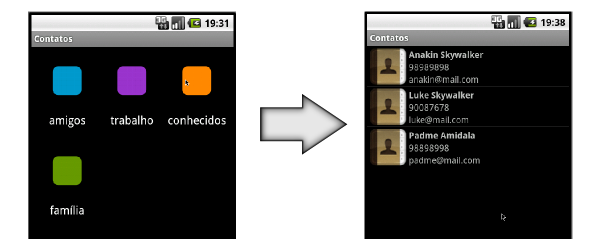
\includegraphics{img/screenshot-grupos.png}
\caption{Tela de Grupos}
\end{figure}

% apêndices
% -- Sobre o Autor
\appendix

\chapter{Sobre o Autor}

Estudante de Ciência da Computação no IFCE Campus Maracanaú, Ceará, Brazil. Programador Java,
PHP, Ruby. Trabalha na Fidias Software, empresa que ajudou a fundar juntamente com José Alberto
e Shara Shami.

\section*{Sugestões e Críticas}

Para fazer sugestões e críticas envie e-mail para \texttt{camurca.home@gmail.com}. Para ficar antenado
no mundo do Software Livre me acompanhe no Twitter:\\ \url{https://twitter.com/#!/atilacamurca}.

\section*{Código-fonte deste guia}

Você pode baixar o código-fonte deste guia em\\ \url{https://github.com/atilacamurca/guia-aberto-android}.

Visite também a página do projeto\\ \url{http://atilacamurca.github.com/guia-aberto-android/} e verifique se
há atualizações.

\printglossary

\end{document}
